\subsection{How is location calculated}
The following sections aim is to cover the different way location is calculated independent of the technologies required to gather the data. As well as provide an insight into the algorithms and general approach to positioning systems such that the system can be implemented. 

\subsubsection{Location classification methods}
Two types of localisation system where found throughout the research, the first of these is a classification system this kind of system can classify a zone/area of a user.
The second kind of system that was identified from research is a co-ordinate based system this system appears more commonly in research, part of this is probably down to the search terms being biased towards accurate positioning systems in order to match the projects aims and objectives. A co-ordinate based system provides a co-ordinate of the user within space. One well known implementation for this is GPS which provides a longitude and latitude of the user \cite{kyes_2017_what}.

With the projects aims and objective to be able to achieve an accurate and robust indoor positioning system. An important factor to consider is the technologies and algorithms which will make this a possibility, hence a focus on coordinate based technologies will be made throughout the rest of the research. However, the cost of the system is significant to consider and using a classification system could allow the cost be reduced, since this kind of system would require one sensor for a given area. Additionally, this system could be implemented into smaller areas where exact location is not required, for example a small office, doing so would not impact the performance of the system. On the other hand, if there are many small zones that need to be classified near to each other it may become more cost effective keep full positioning as more sensor's may be needed to classify individual offices, but this depends on the implementation details of the classification system.  

\subsubsection{General Approach to Location Calculation}
Many technologies used for indoor positioning make use of lateration for calculation of the users location. Lateration is the method of measuring distances from sensor's at a known location. The calculation of the position from the received data is a problem of finding the intersecting area/point of N circles. The most popular method found within research is trilateration which is three distance measurements. \cite{shchekotov_2015_indoor} explains that three circles (see figure \ref{fig:latandang}) is the minimum to achieve point accuracy as anything below this would result in two or more possible locations of the user. Finally turning the signal strength into a distance measurement is done by the Log-normal Distance Path Loss (LDPL) model, \cite{yang_2018_an} paper goes onto explaining how to potentially improve the accuracy to gain a better measurement from the sensor data.
 
\subsubsection{Angulation}
Another method of calculating location is by using angulation, within one method of this within wireless signal approaches is the use of Angle Of Arrival/Angle Of Departure (AoA/AoD). These methods are only supported by a limited range of standards such as Ultra-wide band and Bluetooth 5.1. These methods can work in conjunction with the lateration approaching yielding a significantly more accurate result, (\cite{mysticmedia_2020_the}) and (\cite{lehtimki_bluetooth}) both cover's this principal with Bluetooth 5 and how to use angulation to get the accuracy down to 2cm see Figure \ref{fig:latandang} for a visual of how this works.

\begin{figure}[h]
	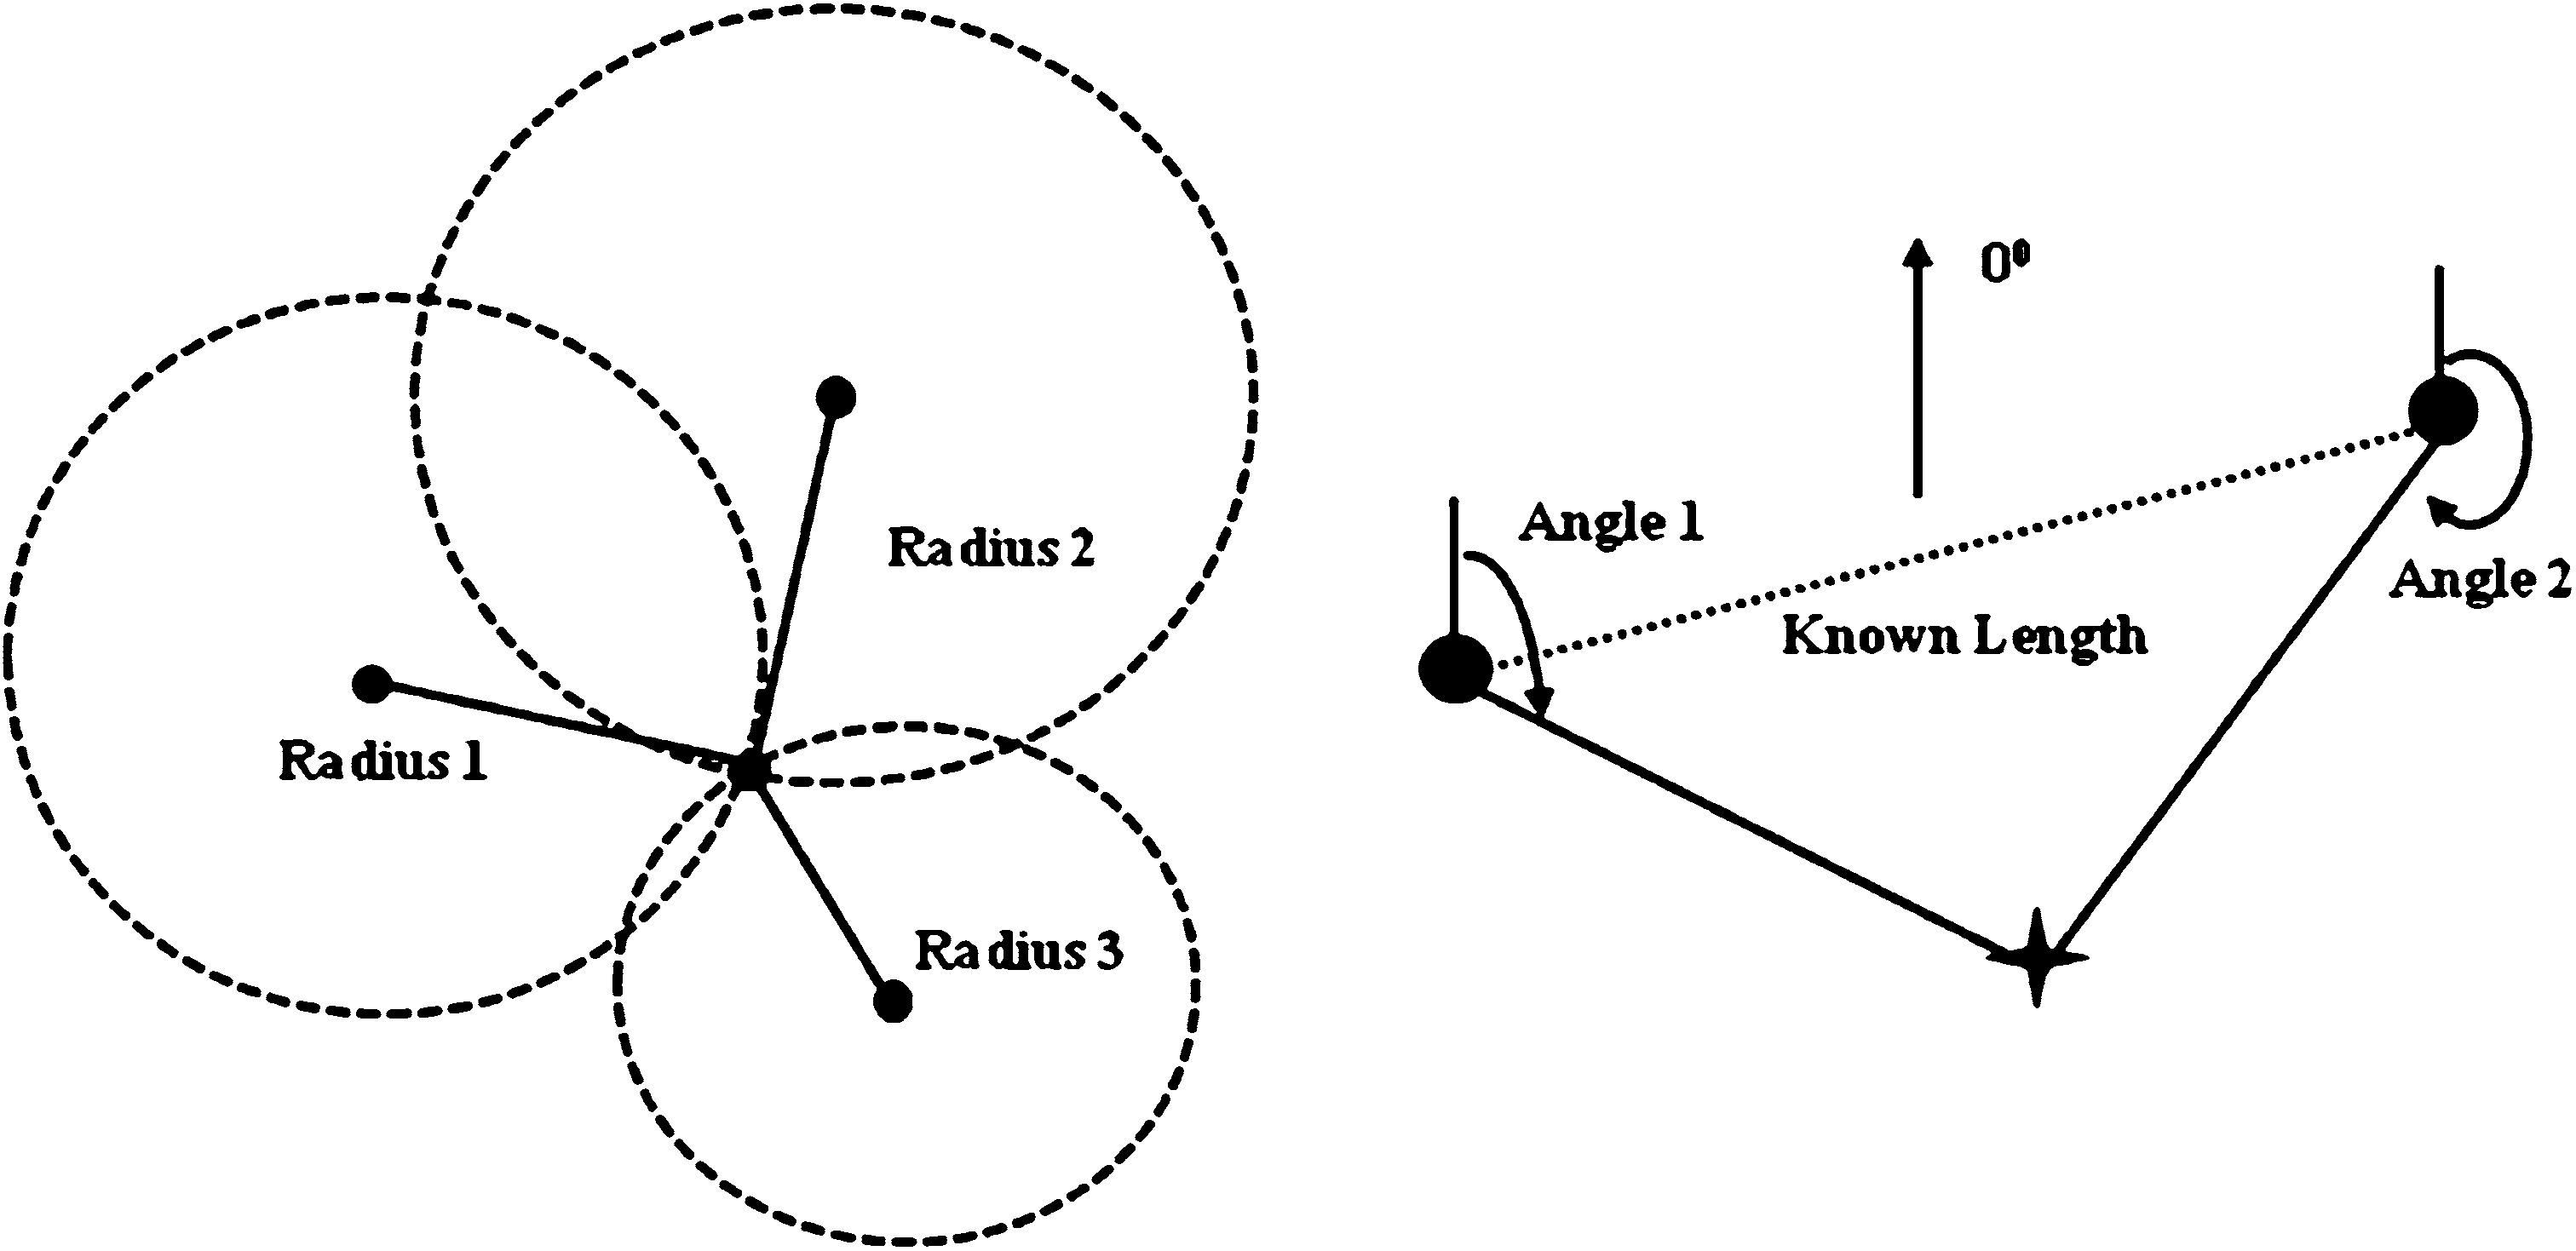
\includegraphics[width=\linewidth]{images/research/distanceandaoa.png}\\
	\caption{how lateration and angulation are converted to a location (\cite{kim_2013_rfidbased})}
	\label{fig:latandang}
\end{figure}

\subsubsection{Accelerometer based positioning}
In addition to the methods above there are other ways of indoor positioning. One of the more interesting methods of this is the use of the phones accelerometer as covered by \cite{nagpalparamvirsingh_2013_indoor}. The paper covers in detail the use of the accelerometer for indoor positioning, showing a range of graphs and figures demonstrating the accuracy of this form system. It was concluded by the paper that accuracy of such a system is adequate. However, over time the accuracy of the system degrades. The system works by using a known initialisation point of the user and calculating a movement based on the accelerometer readings. Other paper's where also found on this method such as the paper by \cite{palma_2017_evolution}, which backs up the first paper's findings. To solve the problem of accuracy degradation over time there is a few solutions, one such solution is to include QR codes at regular points around the real indoor location, when the accuracy is known to be too degraded the user can be prompted to scan one of these codes which will update the system. The paper by \cite{comer_uwb_vs_ble} covers a method called "IMU Sensor Fusion", this methods combines Accelerometer based positioning with lateration approaches. Doing so creates a feedback loop/point of truth which can be used to increase the accuracy of both systems compared to just one separately.

\subsubsection{Other ways of calculating location}
Finally, there also exists other systems that can be used for indoor positioning however they have large pitfalls not making them viable for this project aims and objectives. Some of these include cost, accuracy and requiring a dedicated server. These technologies include Infrared (\cite{palma_2017_evolution}), Ultrasonic (\cite{qi_2017_a}), RFID (\cite{kim_2013_rfidbased}), WiFi (\cite{duyuanfeng_2016_flexible}). It's worth noting that WiFi and RFID based approaches both rely on lation based techniques for these and where not covered within the comparison due to some of the prior mentioned reasons.
